\section{Theory}
\label{sec:Theory}
\subsection{The Sagnac Interferometer}
\label{sec:The_Sagnac_Interferometer}
A Sagnac interferometer is a device built out of multiple mirrors and a polarising beam splitter cube (PBSC). Its purpose is to split a laser beam entering the interferometer into two beams, which can the be redirected over different path. A sketch of the device can be seen in \autoref{fig:interferometer}.\\
To split the beam, it first goes through the PBSC at a $45$ degree angle to the beam. This reflects s-polarised light, while transmitting p-polarised light. The beams then get reflected thrice via multiple mirrors to reenter the PBSC. A portion of each of these beams is then transmitted/reflected into the output area, as shown in \autoref{fig:interferometer}.\\
\begin{figure}
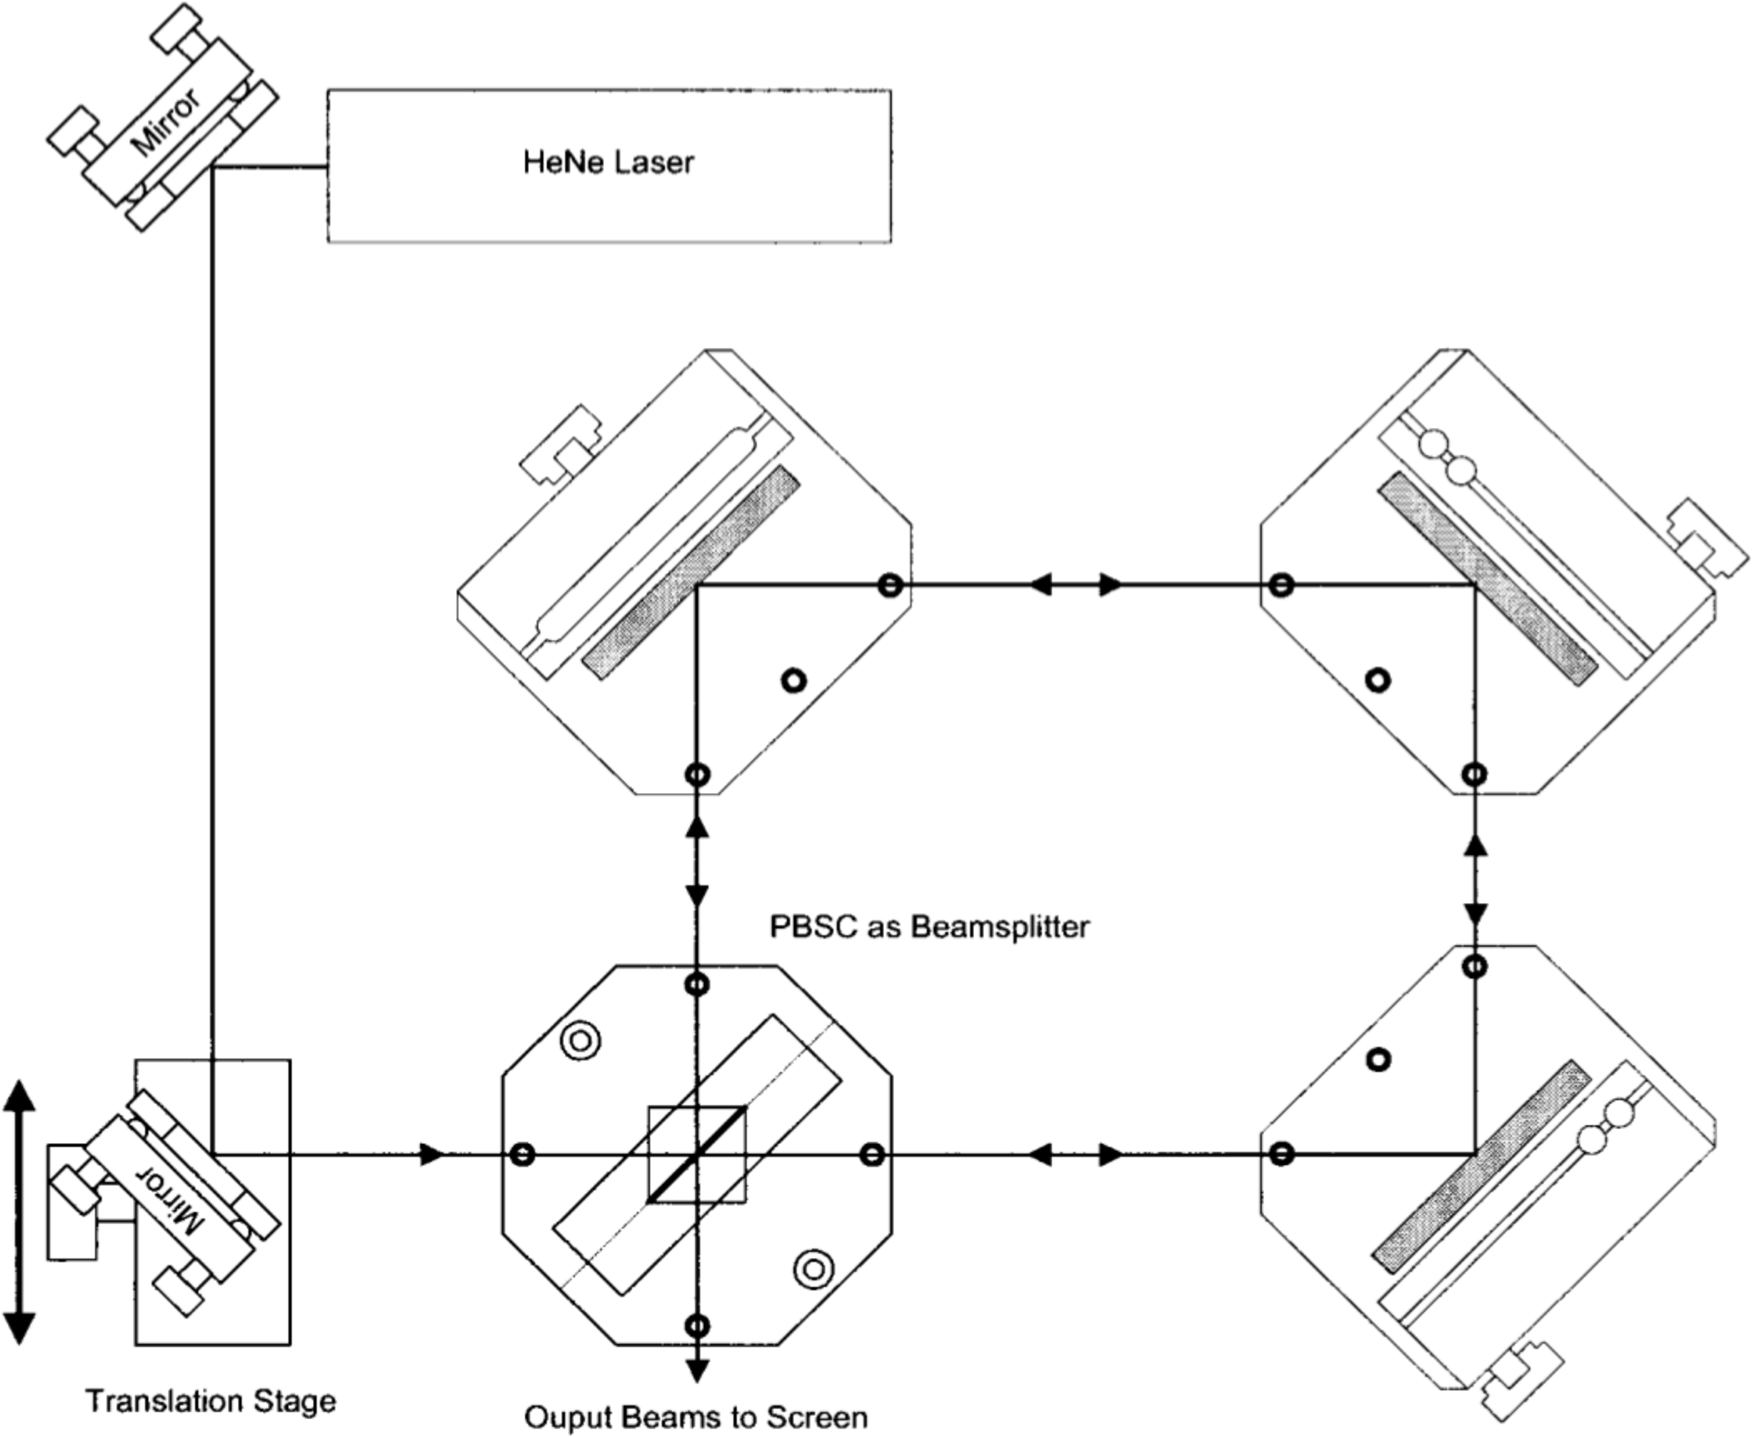
\includegraphics[width=\linewidth]{./figures/aufbau.pdf}
\caption{The Sagnac Interferometer}
\label{fig:interferometer}
\end{figure}
However if the interferometer is perfectly adjusted, the resulting beams will overlap at all stages of the interferometer. To manipulate each beam individually, it is necessary to separate their superposition. To do so the laser, or in this case the mirror between the laser and the mirror, has to be moved in the direction that is shown by the arrow in the picture. Doing so results in the two beams following different paths after entering the PBSC. During this stage, one of the beams can be sent through a medium, making it possible to measure the medium's refraction index.
\\
An important quantity for interferometers is the contrast. The name is self-explanatory: Just like in the case of colours, where the contrast between two colours is highest if they are opposite to each other (for example black and white) and lowest if both colours are the same, the contrast in an interference picture is defined as 
\begin{aquation}
  K &= \frac{I_\text{max}-I_\text{min}}{I_\text{max} + I_\text{min}} \tc
\end{aquation}
with minimal and maximal intensities $I_\text{min}$ and $I_\text{max}$.\\
The closer the contrast is to $1$, the better it is. On the other hand, it is worse the lower it is. The ideal contrast therefore occurs for $I_\text{min}=0$, while the worst case is that there are no minima/maxima, meaning that $I_\text{min}=I_\text{max}$.\\
In this experiment, the contrast will be measured dependent on the phase angle of a polarisation filter that has been positioned in the beam's path. For this, the contrast takes the form 
\begin{aquation}
K &= A|sin(2\varphi + \delta)| \tp
\end{aquation}

\subsection{The Refraction Index}
The refraction index of a medium is a measure for how fast light travels inside that medium. It is manifest in the dispersion relation inside the medium, effectively scaling the speed of light's vacuum value. This means that 
\begin{aquation}
  n &= \frac{c_\text{medium}}{c_\text{vacuum}} \tp 
\end{aquation}
Plugging this into the vacuum dispersion relation, the resulting refraction index inside the medium, depending on the wave number inside the medium, is
\begin{aquation}
  n &= \frac{\lambda_\text{vacuum} k}{2\pi} \tp
\end{aquation}
\subsubsection{Gaseous Medium}
To measure this index, one of the beam is lead through a gas cell. The difference in the speed of light inside the cell yields a phase difference 
\begin{aquation}
  \Delta \varphi &= \frac{2 \pi L}{\lambda_\text{vac}}\Delta n
\end{aquation}
between the two beams, which results in them interfering with each other after being reunited. The number of maxima of interference is proportional to the phase difference. It is 
\begin{aquation}
  M &= \frac{\Delta \varphi}{2 \pi} \tp
\end{aquation}
The Lorentz-Lorenz equation 
\begin{aquation}
  \frac{n^2-1}{n^2+1} &= \frac{N \alpha}{3\epsilon_0}
\end{aquation}
with the particle density $N$.\\
Since the refraction index of a gas is $\approx 1$, it can be expanded, yielding
\begin{aquation}
  n &= \approx \sqrt{1 + \frac{3 A p}{R T}} \tp
\end{aquation}
This means that the refraction index can be measured by varying the gas's pressure and/or temperature.

\subsubsection{Solid Medium}
\begin{figure}
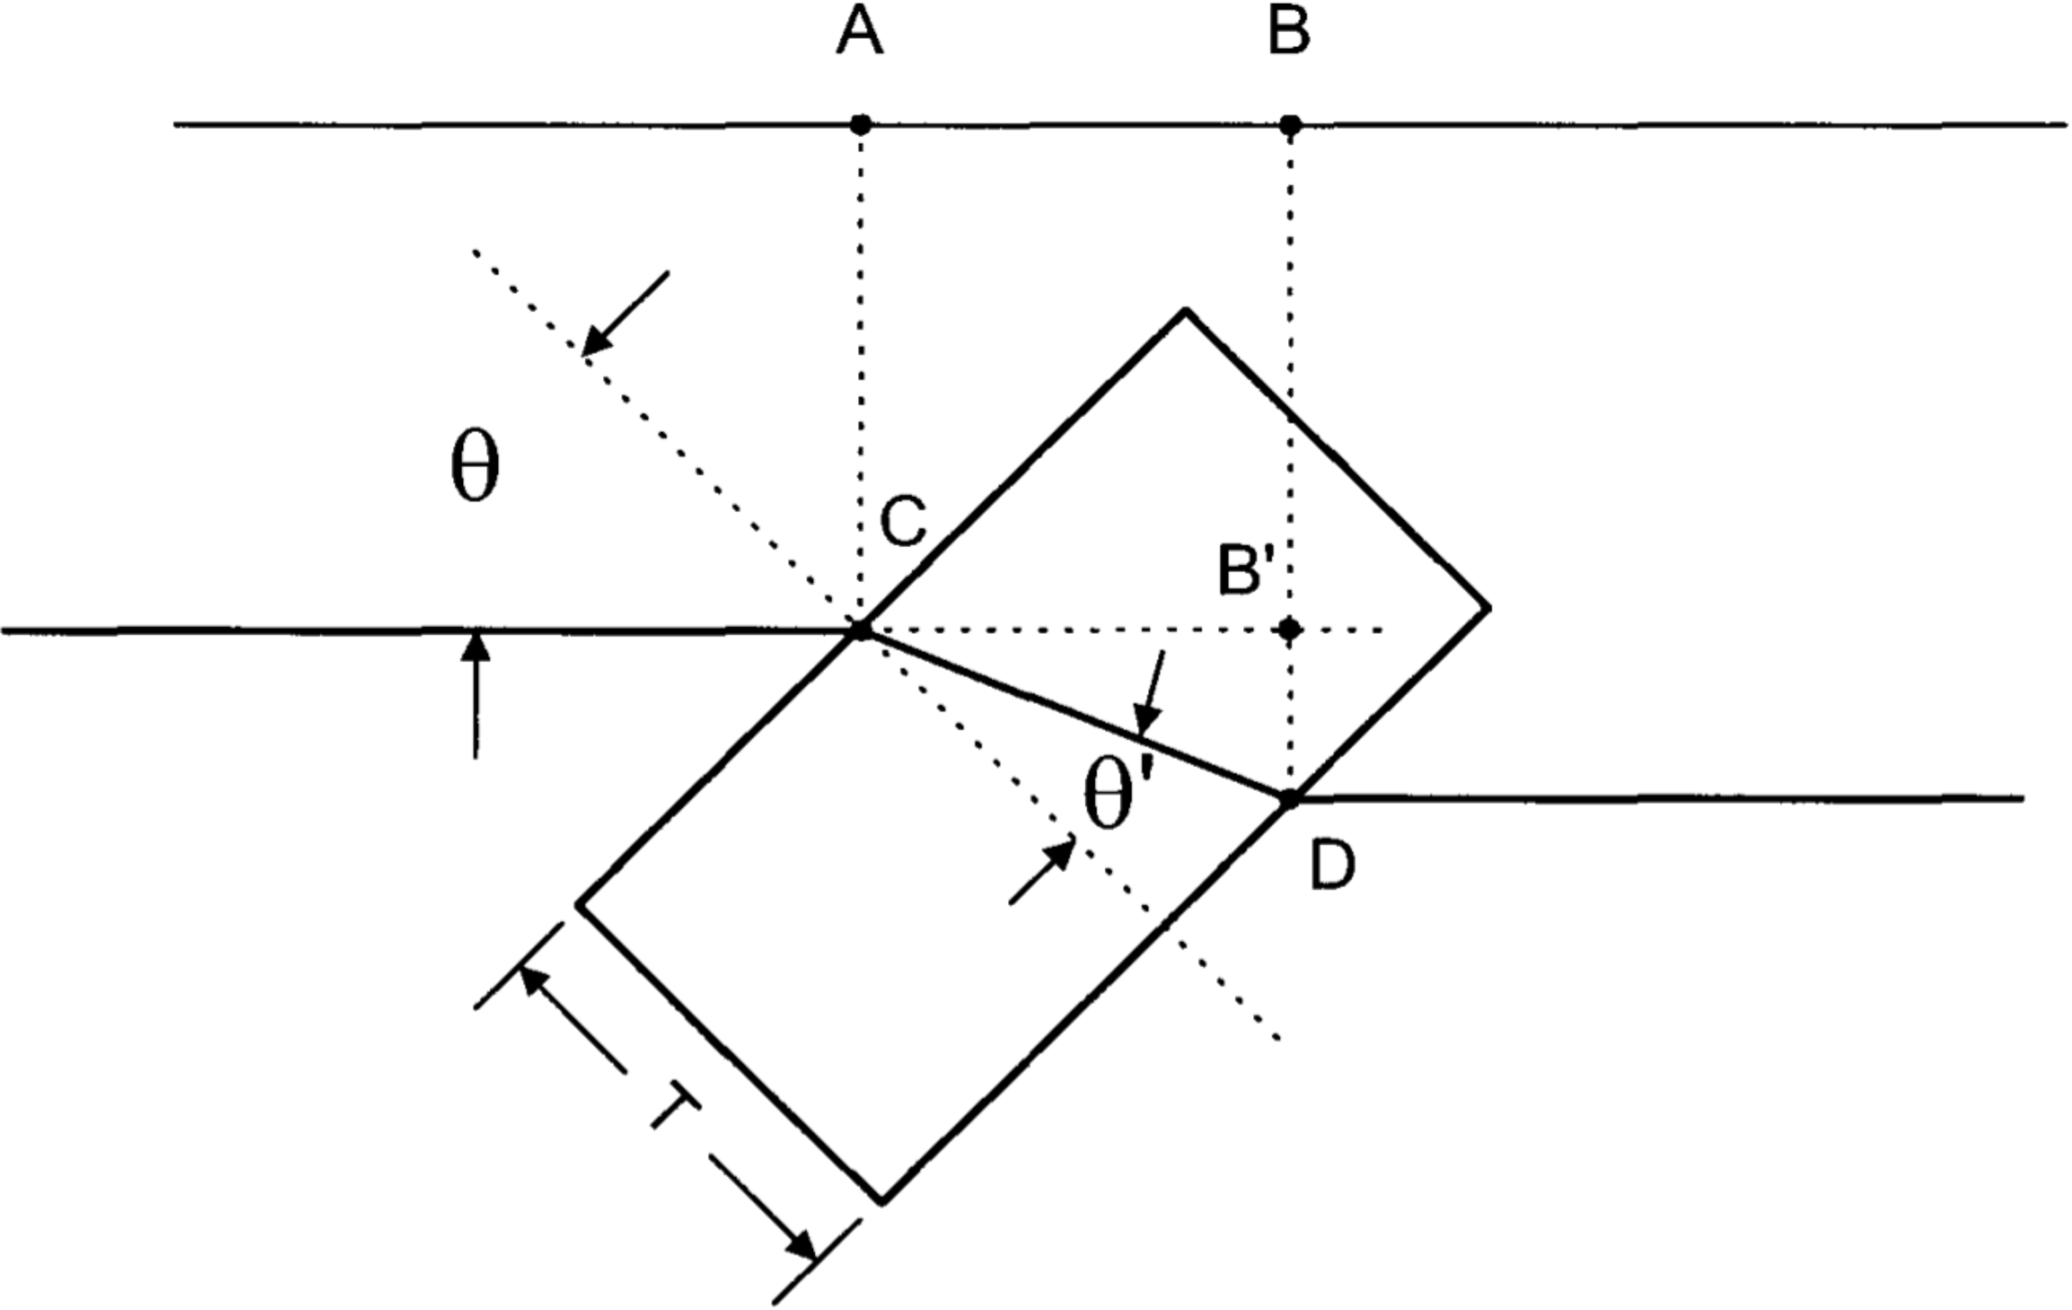
\includegraphics[width=\linewidth]{./figures/glasplaettchen.pdf}
\caption{The geometry of the beam inside a solid medium}
\label{fig:Geometrie}
\end{figure}
A beam of light is refracted when entering a medium. For this reason, the way traveled by the beam that travels through it will be longer than that of the other beam. If the way of the beam outside the medium would be $a$ (between the points A and B, as depicted in \autoref{fig:Geometrie}) and the thickness of the medium be $T$, the way traveled by the beam inside the medium is 
\begin{aquation}
  b &\coloneqq a \cos(\theta^\prime - \theta) \tp
\end{aquation}
With this, the phase difference for a solid body, which can not be determined as easily as with the gas via its pressure and temperature is
\begin{aquation}
\label{eq:phase-difference_solid}
  \Delta \varphi &= \frac{2 \pi}{\lambda_\text{vacuum}} \lbr n_\text{medium} b - a \rbr \\
  		&=v \frac{2 \pi T}{\lambda_\text{vacuum}} \lbr \frac{n-\cos(\theta^\prime - \theta)}{\cos(\theta^\prime)}\rbr \tp
\end{aquation}
The angles are related via Snellius' formula
\begin{aquation}
  n \sin(\theta^\prime) &= \sin(\theta) \tp
\end{aquation}
However in this experiment, the medium has been inserted into both beams. It consisted of two glass plates of identical thickness that were mounted on a rotation holder at an angle of $20$ degrees. For this reason, the refraction indices in the above formula become the same, and the formula can be symmetrised. Going through the previous steps again for each beam, at angles $\theta_\pm \coloneqq \theta \pm \theta_0$, with $\theta_0 = 20 \text{degree}$, the final expression for the number of interference maxima is 
\begin{aquation}
  M &= \frac{T}{\lambda_\text{vacuum}} \lbr \frac{n - \cos\lbr\theta_+ - \arcsin\lbr \frac{\sin(\theta_+)}{n} \rbr\rbr}{\cos\lbr\arcsin\lbr\frac{\sin(\theta_+)}{n}\rbr\rbr} - \frac{n - \cos\lbr\theta_- - \arcsin\lbr \frac{\sin(\theta_-)}{n} \rbr\rbr}{\cos\lbr\arcsin\lbr\frac{\sin(\theta_-)}{n}\rbr\rbr}\rbr
\end{aquation}



